\documentclass[twoside]{book}

% Packages required by doxygen
\usepackage{fixltx2e}
\usepackage{calc}
\usepackage{doxygen}
\usepackage[export]{adjustbox} % also loads graphicx
\usepackage{graphicx}
\usepackage[utf8]{inputenc}
\usepackage{makeidx}
\usepackage{multicol}
\usepackage{multirow}
\PassOptionsToPackage{warn}{textcomp}
\usepackage{textcomp}
\usepackage[nointegrals]{wasysym}
\usepackage[table]{xcolor}

% Font selection
\usepackage[T1]{fontenc}
\usepackage[scaled=.90]{helvet}
\usepackage{courier}
\usepackage{amssymb}
\usepackage{sectsty}
\renewcommand{\familydefault}{\sfdefault}
\allsectionsfont{%
  \fontseries{bc}\selectfont%
  \color{darkgray}%
}
\renewcommand{\DoxyLabelFont}{%
  \fontseries{bc}\selectfont%
  \color{darkgray}%
}
\newcommand{\+}{\discretionary{\mbox{\scriptsize$\hookleftarrow$}}{}{}}

% Page & text layout
\usepackage{geometry}
\geometry{%
  a4paper,%
  top=2.5cm,%
  bottom=2.5cm,%
  left=2.5cm,%
  right=2.5cm%
}
\tolerance=750
\hfuzz=15pt
\hbadness=750
\setlength{\emergencystretch}{15pt}
\setlength{\parindent}{0cm}
\setlength{\parskip}{0.2cm}
\makeatletter
\renewcommand{\paragraph}{%
  \@startsection{paragraph}{4}{0ex}{-1.0ex}{1.0ex}{%
    \normalfont\normalsize\bfseries\SS@parafont%
  }%
}
\renewcommand{\subparagraph}{%
  \@startsection{subparagraph}{5}{0ex}{-1.0ex}{1.0ex}{%
    \normalfont\normalsize\bfseries\SS@subparafont%
  }%
}
\makeatother

% Headers & footers
\usepackage{fancyhdr}
\pagestyle{fancyplain}
\fancyhead[LE]{\fancyplain{}{\bfseries\thepage}}
\fancyhead[CE]{\fancyplain{}{}}
\fancyhead[RE]{\fancyplain{}{\bfseries\leftmark}}
\fancyhead[LO]{\fancyplain{}{\bfseries\rightmark}}
\fancyhead[CO]{\fancyplain{}{}}
\fancyhead[RO]{\fancyplain{}{\bfseries\thepage}}
\fancyfoot[LE]{\fancyplain{}{}}
\fancyfoot[CE]{\fancyplain{}{}}
\fancyfoot[RE]{\fancyplain{}{\bfseries\scriptsize Generated on Thu Jul 23 2015 22\+:15\+:29 for Wave Equation by Doxygen }}
\fancyfoot[LO]{\fancyplain{}{\bfseries\scriptsize Generated on Thu Jul 23 2015 22\+:15\+:29 for Wave Equation by Doxygen }}
\fancyfoot[CO]{\fancyplain{}{}}
\fancyfoot[RO]{\fancyplain{}{}}
\renewcommand{\footrulewidth}{0.4pt}
\renewcommand{\chaptermark}[1]{%
  \markboth{#1}{}%
}
\renewcommand{\sectionmark}[1]{%
  \markright{\thesection\ #1}%
}

% Indices & bibliography
\usepackage{natbib}
\usepackage[titles]{tocloft}
\setcounter{tocdepth}{3}
\setcounter{secnumdepth}{5}
\makeindex

% Custom commands
\newcommand{\clearemptydoublepage}{%
  \newpage{\pagestyle{empty}\cleardoublepage}%
}


%===== C O N T E N T S =====

\begin{document}

% Titlepage & ToC
\pagenumbering{roman}
\begin{titlepage}
\vspace*{7cm}
\begin{center}%
{\Large Wave Equation \\[1ex]\large 0.\+0 }\\
\vspace*{1cm}
{\large Generated by Doxygen 1.8.9.1}\\
\vspace*{0.5cm}
{\small Thu Jul 23 2015 22:15:29}\\
\end{center}
\end{titlepage}
\clearemptydoublepage
\tableofcontents
\clearemptydoublepage
\pagenumbering{arabic}

%--- Begin generated contents ---
\chapter{Wave\+Equation}
\label{md__home_cfadden3__git_hub__wave_equation__r_e_a_d_m_e}
C++ implementation of a 2\+D parallel wave equation solver using multiresolution analysis 
\chapter{Hierarchical Index}
\section{Class Hierarchy}
This inheritance list is sorted roughly, but not completely, alphabetically\+:\begin{DoxyCompactList}
\item \contentsline{section}{Grid}{\pageref{class_grid}}{}
\begin{DoxyCompactList}
\item \contentsline{section}{Field}{\pageref{class_field}}{}
\end{DoxyCompactList}
\item \contentsline{section}{Gui\+Main}{\pageref{class_gui_main}}{}
\item J\+Frame\begin{DoxyCompactList}
\item \contentsline{section}{Gui}{\pageref{class_gui}}{}
\end{DoxyCompactList}
\item Action\+Listener\begin{DoxyCompactList}
\item \contentsline{section}{Gui}{\pageref{class_gui}}{}
\end{DoxyCompactList}
\end{DoxyCompactList}

\chapter{Class Index}
\section{Class List}
Here are the classes, structs, unions and interfaces with brief descriptions\+:\begin{DoxyCompactList}
\item\contentsline{section}{{\bf Field} }{\pageref{class_field}}{}
\item\contentsline{section}{{\bf Grid} }{\pageref{class_grid}}{}
\item\contentsline{section}{{\bf Gui} }{\pageref{class_gui}}{}
\item\contentsline{section}{{\bf Gui\+Main} }{\pageref{class_gui_main}}{}
\end{DoxyCompactList}

\chapter{File Index}
\section{File List}
Here is a list of all documented files with brief descriptions\+:\begin{DoxyCompactList}
\item\contentsline{section}{/home/cfadden3/\+Git\+Hub/\+Wave\+Equation/gui/{\bf Gui.\+java} \\*G\+U\+I implementation for electromagnetic simulations }{\pageref{_gui_8java}}{}
\item\contentsline{section}{/home/cfadden3/\+Git\+Hub/\+Wave\+Equation/include/{\bf Field.\+h} \\*Class definition of the wave equation field }{\pageref{_field_8h}}{}
\item\contentsline{section}{/home/cfadden3/\+Git\+Hub/\+Wave\+Equation/include/{\bf Grid.\+h} \\*Class definition for global electromagnetics grid }{\pageref{_grid_8h}}{}
\end{DoxyCompactList}

\chapter{Class Documentation}
\section{Field Class Reference}
\label{class_field}\index{Field@{Field}}
Inheritance diagram for Field\+:\begin{figure}[H]
\begin{center}
\leavevmode
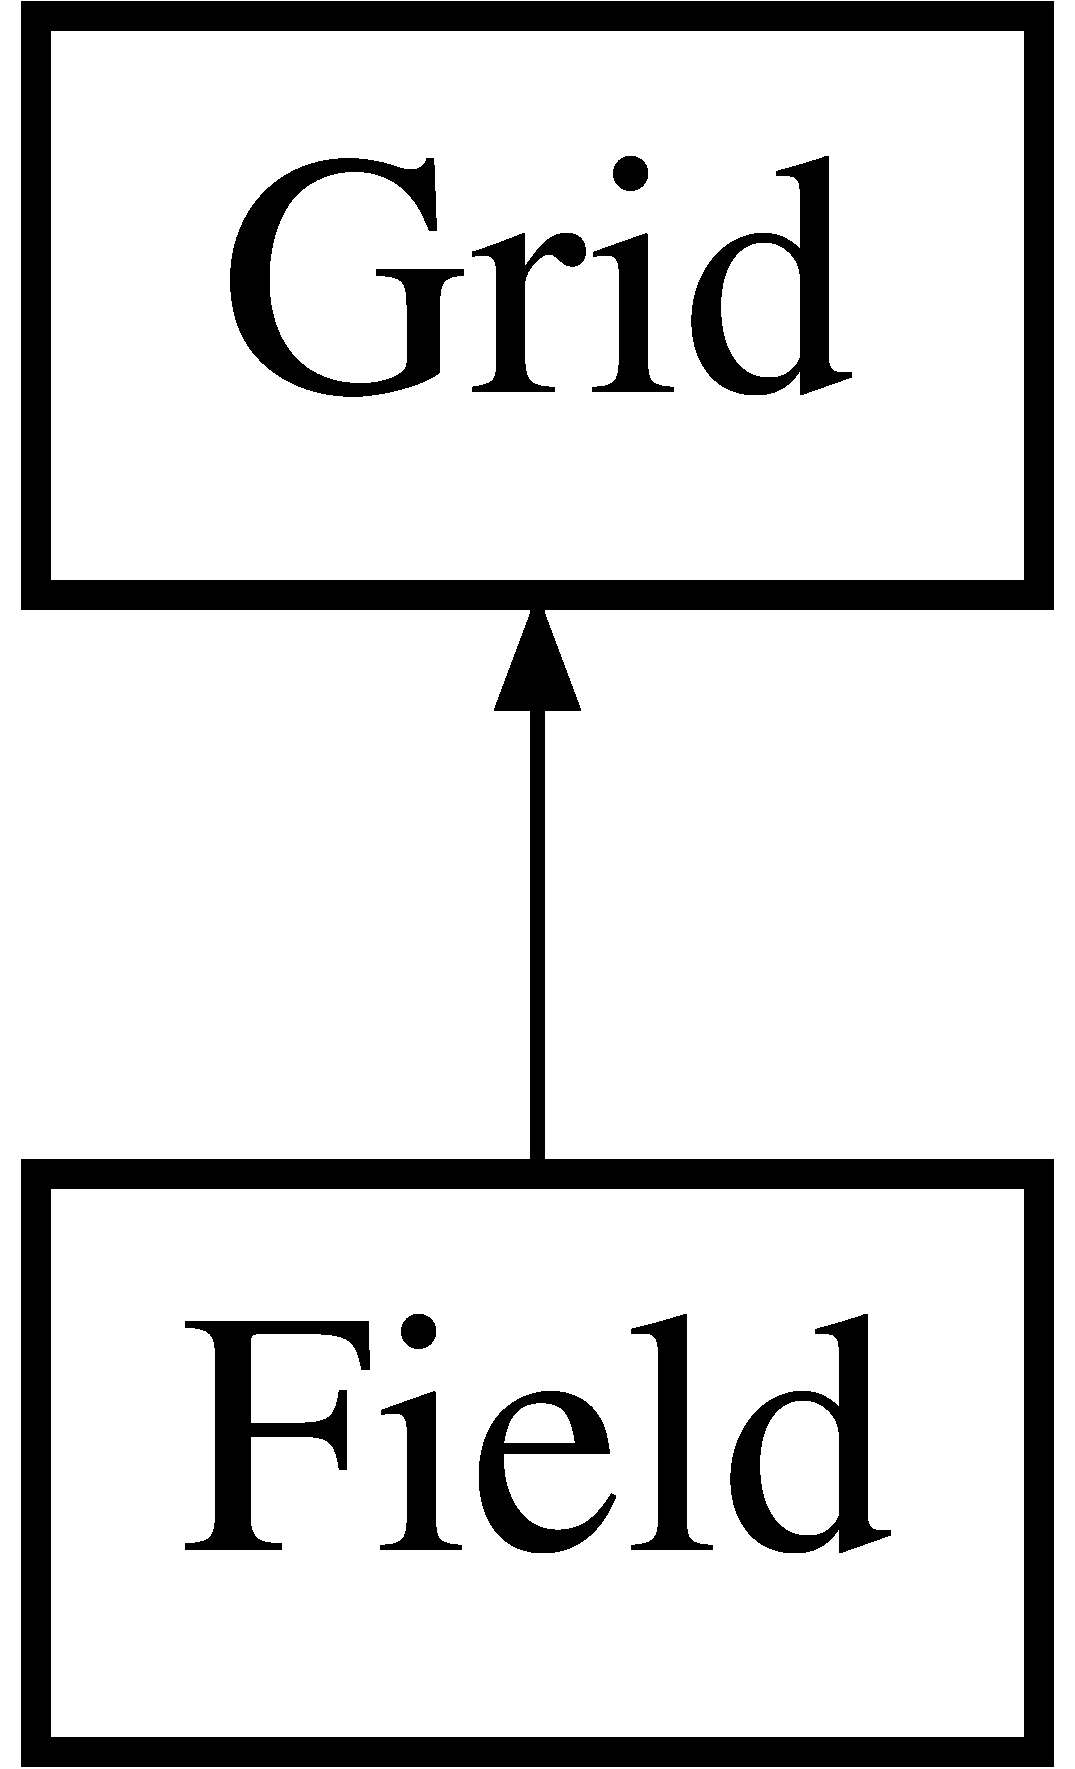
\includegraphics[height=2.000000cm]{class_field}
\end{center}
\end{figure}
\subsection*{Public Member Functions}
\begin{DoxyCompactItemize}
\item 
{\bf Field} ()
\begin{DoxyCompactList}\small\item\em Constructor of the \doxyref{Field}{p.}{class_field} class. \end{DoxyCompactList}\item 
void {\bf Update} (int)
\begin{DoxyCompactList}\small\item\em Updates the field value. \end{DoxyCompactList}\item 
double {\bf Source} (int)
\begin{DoxyCompactList}\small\item\em Returns the source function value. \end{DoxyCompactList}\item 
void {\bf Print} ()
\begin{DoxyCompactList}\small\item\em Outputs the field values. \end{DoxyCompactList}\item 
double {\bfseries Dim2} (int, int)\label{class_field_a38a060a3037f15811edd713451f5b5f7}

\item 
double \& {\bfseries Az\+Old} (int, int)\label{class_field_aae833bb003bd88826447a6a99e6f1e8e}

\item 
double \& {\bfseries Az\+New} (int, int)\label{class_field_ab7e9bc608b5ef944e00e64ac87e9476a}

\item 
double \& {\bfseries Az} (int, int)\label{class_field_ad06425d1d3a675a040d47ff5daeec316}

\item 
double \& {\bfseries Ca} (int, int)\label{class_field_a4aa353e182867290e3e4b80c49e79497}

\end{DoxyCompactItemize}
\subsection*{Additional Inherited Members}


\subsection{Constructor \& Destructor Documentation}
\index{Field@{Field}!Field@{Field}}
\index{Field@{Field}!Field@{Field}}
\subsubsection[{Field}]{\setlength{\rightskip}{0pt plus 5cm}Field\+::\+Field (
\begin{DoxyParamCaption}
{}
\end{DoxyParamCaption}
)}\label{class_field_a3e804c92273d9159f413f227b535c672}


Constructor of the \doxyref{Field}{p.}{class_field} class. 

The field is initialized with values from the inheritance of the \doxyref{Grid}{p.}{class_grid}. Its values therefore depend on the default constructor of the \doxyref{Grid}{p.}{class_grid}. 

\subsection{Member Function Documentation}
\index{Field@{Field}!Print@{Print}}
\index{Print@{Print}!Field@{Field}}
\subsubsection[{Print}]{\setlength{\rightskip}{0pt plus 5cm}void Field\+::\+Print (
\begin{DoxyParamCaption}
{}
\end{DoxyParamCaption}
)}\label{class_field_a318ede8c868e024ed2ede4c0bc6e5058}


Outputs the field values. 

This function prints the values of the field at all points to a csv file, so the results can be seen graphically. \index{Field@{Field}!Source@{Source}}
\index{Source@{Source}!Field@{Field}}
\subsubsection[{Source}]{\setlength{\rightskip}{0pt plus 5cm}double Field\+::\+Source (
\begin{DoxyParamCaption}
\item[{int}]{t}
\end{DoxyParamCaption}
)}\label{class_field_a2d3017d92f34b4e4a9e1474bb231da64}


Returns the source function value. 

This returns the value of the source, either gaussian or sine, and uses that to input power into the grid.


\begin{DoxyParams}{Parameters}
{\em t} & the current time \\
\hline
\end{DoxyParams}
\begin{DoxyReturn}{Returns}
the value of the source 
\end{DoxyReturn}
\index{Field@{Field}!Update@{Update}}
\index{Update@{Update}!Field@{Field}}
\subsubsection[{Update}]{\setlength{\rightskip}{0pt plus 5cm}void Field\+::\+Update (
\begin{DoxyParamCaption}
\item[{int}]{t}
\end{DoxyParamCaption}
)}\label{class_field_a7159f10e4abd87a193ef5a17da01a5ef}


Updates the field value. 

This function is in the time loop, and updates the field value using finite differences.


\begin{DoxyParams}{Parameters}
{\em n} & the current number of iterations \\
\hline
\end{DoxyParams}
\begin{DoxyReturn}{Returns}
The field value is updated 
\end{DoxyReturn}


The documentation for this class was generated from the following files\+:\begin{DoxyCompactItemize}
\item 
/home/cfadden3/\+Git\+Hub/\+Wave\+Equation/include/{\bf Field.\+h}\item 
/home/cfadden3/\+Git\+Hub/\+Wave\+Equation/src/Field.\+cpp\end{DoxyCompactItemize}

\section{Grid Class Reference}
\label{class_grid}\index{Grid@{Grid}}
Inheritance diagram for Grid\+:\begin{figure}[H]
\begin{center}
\leavevmode
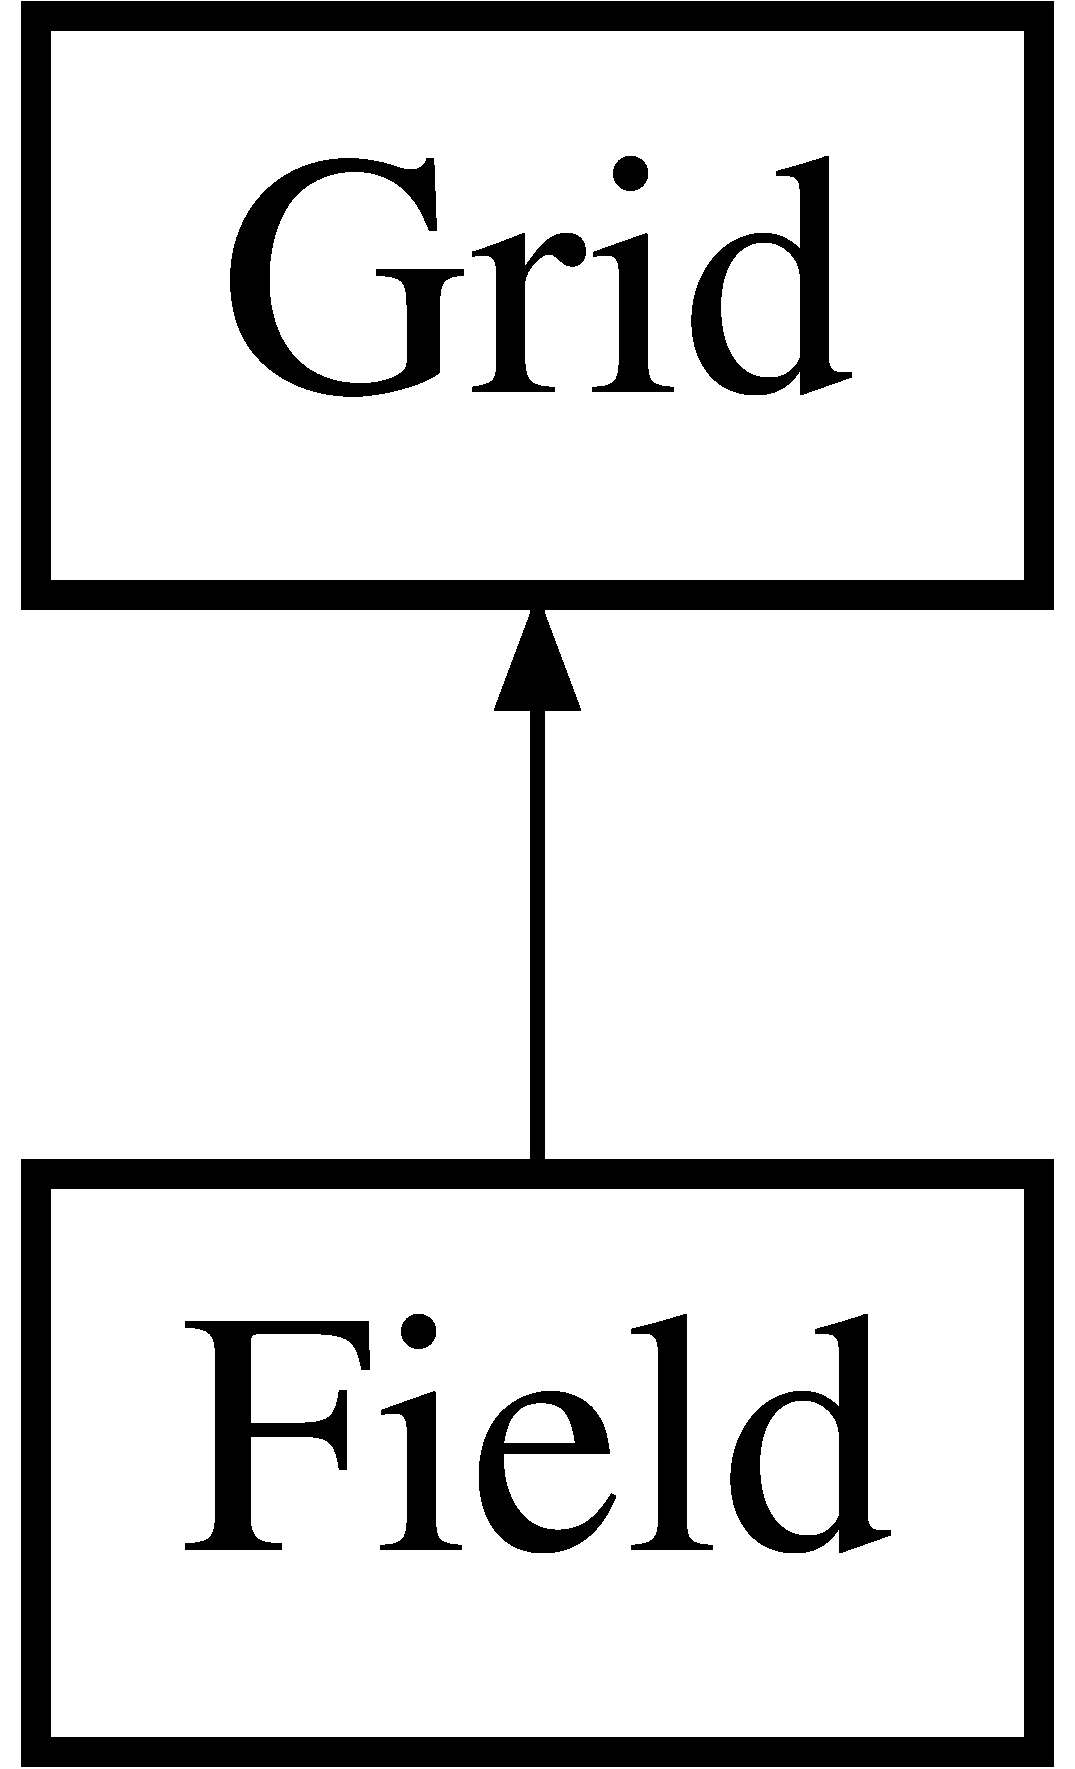
\includegraphics[height=2.000000cm]{class_grid}
\end{center}
\end{figure}
\subsection*{Public Member Functions}
\begin{DoxyCompactItemize}
\item 
{\bf Grid} ()
\begin{DoxyCompactList}\small\item\em Constructor of the \doxyref{Grid}{p.}{class_grid} class. \end{DoxyCompactList}\item 
int {\bf get\+Max\+Time} ()
\begin{DoxyCompactList}\small\item\em returns the maximum time of simulation \end{DoxyCompactList}\end{DoxyCompactItemize}
\subsection*{Protected Types}
\begin{DoxyCompactItemize}
\item 
enum {\bfseries Source} \{ {\bfseries H\+A\+R\+M\+O\+N\+I\+C}, 
{\bfseries G\+A\+U\+S\+S\+I\+A\+N}
 \}\label{class_grid_abbf91d99a10389a676b2ae4683c41f3d}

\end{DoxyCompactItemize}
\subsection*{Protected Member Functions}
\begin{DoxyCompactItemize}
\item 
double {\bf Harmonic\+Source} (int)
\begin{DoxyCompactList}\small\item\em Returns value of the harmonic source. \end{DoxyCompactList}\item 
double {\bf Gaussian\+Source} (int)
\begin{DoxyCompactList}\small\item\em Returns value of the gaussian source. \end{DoxyCompactList}\end{DoxyCompactItemize}
\subsection*{Protected Attributes}
\begin{DoxyCompactItemize}
\item 
int {\bfseries Size\+X}\label{class_grid_a0624ee310d63ed75758ba1be4640ce9d}

\item 
int {\bfseries Size\+Y}\label{class_grid_adbc706daa9218d1ee9e37feee6a62fbd}

\item 
int {\bfseries t} = 0\label{class_grid_a2dd507d805da86cfdc51034c5c098b7d}

\item 
int {\bfseries Max\+Time}\label{class_grid_ab5143fda0e0c599b2ac46b4588d77c98}

\item 
int {\bf isrc}
\item 
int {\bf jsrc}
\item 
const int {\bfseries cc} = 299792458\label{class_grid_a7e3bb460744596f2df7ea838be8483f6}

\item 
const double {\bfseries mu0} = 16 $\ast$ atan(1) $\ast$ 1.\+0e-\/7\label{class_grid_a5de990921f607452dd11372e4881d959}

\item 
const double {\bfseries eps0} = 1.\+0 / (cc $\ast$ cc $\ast$ mu0)\label{class_grid_acb75b851ea554b4f279e232b94fdff6c}

\item 
double {\bfseries dx}\label{class_grid_a1f52441a37442b054bf153cc362cf2d8}

\item 
double {\bfseries dy}\label{class_grid_ac388777840b30765f83a8a135d7b0cec}

\item 
double {\bfseries dt}\label{class_grid_a8aa332bcbd08178a499c6208e6cba073}

\item 
Source {\bfseries src}\label{class_grid_af4f38a38e63bc28d44b8968a3ecff1b7}

\item 
double {\bfseries freq}\label{class_grid_a273377dfb22fdfb33543bd467c7cdb76}

\item 
std\+::vector$<$ double $>$ {\bfseries epsr}\label{class_grid_ae026e1830e2fc67be14a5c6ce6bba5dd}

\item 
std\+::vector$<$ double $>$ {\bfseries mur}\label{class_grid_acdbfd6bf3f1abbbb988662f2fe986bed}

\end{DoxyCompactItemize}


\subsection{Constructor \& Destructor Documentation}
\index{Grid@{Grid}!Grid@{Grid}}
\index{Grid@{Grid}!Grid@{Grid}}
\subsubsection[{Grid}]{\setlength{\rightskip}{0pt plus 5cm}Grid\+::\+Grid (
\begin{DoxyParamCaption}
{}
\end{DoxyParamCaption}
)}\label{class_grid_a4ac9ff4f63552b4c61ff90fcb35ad66c}


Constructor of the \doxyref{Grid}{p.}{class_grid} class. 

The grid is initialized using values taken from the file created by the Java G\+U\+I. Please take note of the main python script used to run this, and keep in mind the filename is hardcoded at this time. 

\subsection{Member Function Documentation}
\index{Grid@{Grid}!Gaussian\+Source@{Gaussian\+Source}}
\index{Gaussian\+Source@{Gaussian\+Source}!Grid@{Grid}}
\subsubsection[{Gaussian\+Source}]{\setlength{\rightskip}{0pt plus 5cm}double Grid\+::\+Gaussian\+Source (
\begin{DoxyParamCaption}
\item[{int}]{t}
\end{DoxyParamCaption}
)\hspace{0.3cm}{\ttfamily [protected]}}\label{class_grid_a6c07db06db902d014a2fd6620186dbc3}


Returns value of the gaussian source. 

This evaluates a gaussian source, an exponential raised to the \$x$^\wedge$2\$. This has the benefit in a time domain simulation of having multiple frequency components, and therefore can give a more broadband response for the simulation


\begin{DoxyParams}{Parameters}
{\em t} & the time at which to evaluate the function \\
\hline
\end{DoxyParams}
\begin{DoxyReturn}{Returns}
the value at the specified time 
\end{DoxyReturn}
\index{Grid@{Grid}!get\+Max\+Time@{get\+Max\+Time}}
\index{get\+Max\+Time@{get\+Max\+Time}!Grid@{Grid}}
\subsubsection[{get\+Max\+Time}]{\setlength{\rightskip}{0pt plus 5cm}int Grid\+::get\+Max\+Time (
\begin{DoxyParamCaption}
{}
\end{DoxyParamCaption}
)}\label{class_grid_ade2d3195c5ca78f5944011767879aef4}


returns the maximum time of simulation 

This ensures protection of the \doxyref{Grid}{p.}{class_grid} class variables, and acts as a get function for the main program \index{Grid@{Grid}!Harmonic\+Source@{Harmonic\+Source}}
\index{Harmonic\+Source@{Harmonic\+Source}!Grid@{Grid}}
\subsubsection[{Harmonic\+Source}]{\setlength{\rightskip}{0pt plus 5cm}double Grid\+::\+Harmonic\+Source (
\begin{DoxyParamCaption}
\item[{int}]{t}
\end{DoxyParamCaption}
)\hspace{0.3cm}{\ttfamily [protected]}}\label{class_grid_aa676b212b88dc05a81fa8b2824c39ffd}


Returns value of the harmonic source. 

This evaluates a harmonic source, a sine wave, at the specified time, and returns that value. This has a single frequency content, and is mostly used for testing purposes.


\begin{DoxyParams}{Parameters}
{\em t} & the time at which to evaluate the function \\
\hline
\end{DoxyParams}
\begin{DoxyReturn}{Returns}
the value at the specified time 
\end{DoxyReturn}


\subsection{Member Data Documentation}
\index{Grid@{Grid}!isrc@{isrc}}
\index{isrc@{isrc}!Grid@{Grid}}
\subsubsection[{isrc}]{\setlength{\rightskip}{0pt plus 5cm}int Grid\+::isrc\hspace{0.3cm}{\ttfamily [protected]}}\label{class_grid_afea0374c458d210f2f587dadf7ce50cd}
x-\/coordinate of the source on the grid \index{Grid@{Grid}!jsrc@{jsrc}}
\index{jsrc@{jsrc}!Grid@{Grid}}
\subsubsection[{jsrc}]{\setlength{\rightskip}{0pt plus 5cm}int Grid\+::jsrc\hspace{0.3cm}{\ttfamily [protected]}}\label{class_grid_a3ff660de7dea4644d36b0a1dac08c24c}
y-\/coordinate of the source on the grid 

The documentation for this class was generated from the following files\+:\begin{DoxyCompactItemize}
\item 
/home/cfadden3/\+Git\+Hub/\+Wave\+Equation/include/{\bf Grid.\+h}\item 
/home/cfadden3/\+Git\+Hub/\+Wave\+Equation/src/Grid.\+cpp\end{DoxyCompactItemize}

\section{Gui Class Reference}
\label{class_gui}\index{Gui@{Gui}}
Inheritance diagram for Gui\+:\begin{figure}[H]
\begin{center}
\leavevmode
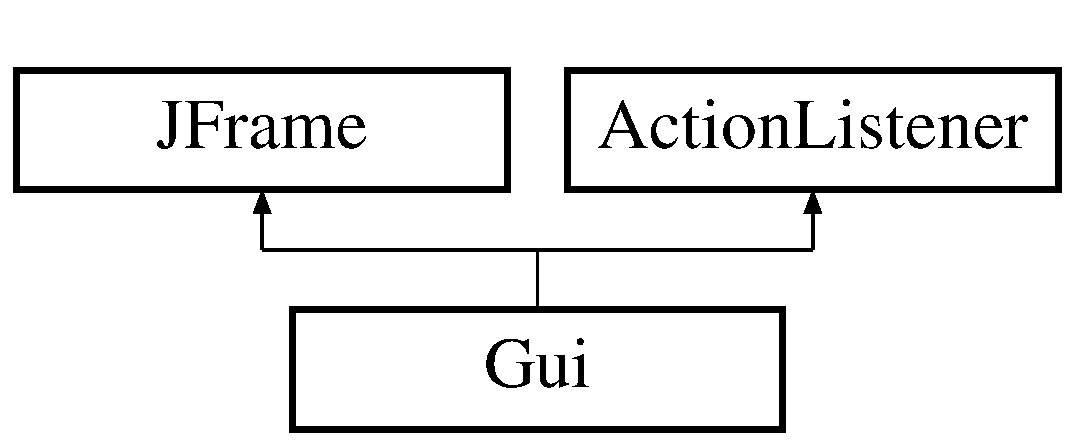
\includegraphics[height=2.000000cm]{class_gui}
\end{center}
\end{figure}
\subsection*{Public Member Functions}
\begin{DoxyCompactItemize}
\item 
{\bf Gui} ()
\begin{DoxyCompactList}\small\item\em Constructor the G\+U\+I class. \end{DoxyCompactList}\item 
void {\bf action\+Performed} (Action\+Event event)
\begin{DoxyCompactList}\small\item\em Done button event handler. \end{DoxyCompactList}\item 
void {\bfseries print\+To\+File} ()\label{class_gui_a610ede38d94e35bda5e50a11b5051392}

\end{DoxyCompactItemize}
\subsection*{Static Public Attributes}
\begin{DoxyCompactItemize}
\item 
static J\+Panel {\bfseries panel}\label{class_gui_a12f024ecd7aabe02ccc79e8f01977d89}

\end{DoxyCompactItemize}


\subsection{Constructor \& Destructor Documentation}
\index{Gui@{Gui}!Gui@{Gui}}
\index{Gui@{Gui}!Gui@{Gui}}
\subsubsection[{Gui}]{\setlength{\rightskip}{0pt plus 5cm}Gui.\+Gui (
\begin{DoxyParamCaption}
{}
\end{DoxyParamCaption}
)\hspace{0.3cm}{\ttfamily [inline]}}\label{class_gui_aa803177c18d790a882ffcbae64b7ebbf}


Constructor the G\+U\+I class. 

This uses the Grid\+Bag\+Layout to arrange textboxes for input to electromagnetic simulations. Default values are set, and the user can choose to modify whichever parameters are preferred. 

\subsection{Member Function Documentation}
\index{Gui@{Gui}!action\+Performed@{action\+Performed}}
\index{action\+Performed@{action\+Performed}!Gui@{Gui}}
\subsubsection[{action\+Performed}]{\setlength{\rightskip}{0pt plus 5cm}void Gui.\+action\+Performed (
\begin{DoxyParamCaption}
\item[{Action\+Event}]{event}
\end{DoxyParamCaption}
)\hspace{0.3cm}{\ttfamily [inline]}}\label{class_gui_ae7af56b42eaf5d12959df7f073280bc3}


Done button event handler. 

When the Done button is pushed, the current value in the textbox is taken, and then printed to a file. 

The documentation for this class was generated from the following file\+:\begin{DoxyCompactItemize}
\item 
/home/cfadden3/\+Git\+Hub/\+Wave\+Equation/gui/{\bf Gui.\+java}\end{DoxyCompactItemize}

\section{Gui\+Main Class Reference}
\label{class_gui_main}\index{Gui\+Main@{Gui\+Main}}
\subsection*{Static Public Member Functions}
\begin{DoxyCompactItemize}
\item 
static void {\bfseries main} (String[$\,$] args)\label{class_gui_main_a78779debd17ffbb0a8ded52d503a08a0}

\end{DoxyCompactItemize}


The documentation for this class was generated from the following file\+:\begin{DoxyCompactItemize}
\item 
/home/cfadden3/\+Git\+Hub/\+Wave\+Equation/gui/Gui\+Main.\+java\end{DoxyCompactItemize}

\chapter{File Documentation}
\section{/home/cfadden3/\+Git\+Hub/\+Wave\+Equation/gui/\+Gui.java File Reference}
\label{_gui_8java}\index{/home/cfadden3/\+Git\+Hub/\+Wave\+Equation/gui/\+Gui.\+java@{/home/cfadden3/\+Git\+Hub/\+Wave\+Equation/gui/\+Gui.\+java}}


G\+U\+I implementation for electromagnetic simulations.  


\subsection*{Classes}
\begin{DoxyCompactItemize}
\item 
class {\bf Gui}
\end{DoxyCompactItemize}


\subsection{Detailed Description}
G\+U\+I implementation for electromagnetic simulations. 

\begin{DoxyAuthor}{Author}
Chris Fadden 
\end{DoxyAuthor}

\section{/home/cfadden3/\+Git\+Hub/\+Wave\+Equation/include/\+Field.h File Reference}
\label{_field_8h}\index{/home/cfadden3/\+Git\+Hub/\+Wave\+Equation/include/\+Field.\+h@{/home/cfadden3/\+Git\+Hub/\+Wave\+Equation/include/\+Field.\+h}}


Class definition of the wave equation field.  


{\ttfamily \#include \char`\"{}Grid.\+h\char`\"{}}\\*
\subsection*{Classes}
\begin{DoxyCompactItemize}
\item 
class {\bf Field}
\end{DoxyCompactItemize}


\subsection{Detailed Description}
Class definition of the wave equation field. 

\begin{DoxyAuthor}{Author}
Chris Fadden 
\end{DoxyAuthor}

\section{/home/cfadden3/\+Git\+Hub/\+Wave\+Equation/include/\+Grid.h File Reference}
\label{_grid_8h}\index{/home/cfadden3/\+Git\+Hub/\+Wave\+Equation/include/\+Grid.\+h@{/home/cfadden3/\+Git\+Hub/\+Wave\+Equation/include/\+Grid.\+h}}


Class definition for global electromagnetics grid.  


{\ttfamily \#include $<$cmath$>$}\\*
{\ttfamily \#include $<$vector$>$}\\*
{\ttfamily \#include $<$string$>$}\\*
\subsection*{Classes}
\begin{DoxyCompactItemize}
\item 
class {\bf Grid}
\end{DoxyCompactItemize}


\subsection{Detailed Description}
Class definition for global electromagnetics grid. 

\begin{DoxyAuthor}{Author}
Chris Fadden 
\end{DoxyAuthor}

%--- End generated contents ---

% Index
\backmatter
\newpage
\phantomsection
\clearemptydoublepage
\addcontentsline{toc}{chapter}{Index}
\printindex

\end{document}
